\documentclass[a4paper]{standalone}
\usepackage{amsmath}
\usepackage{circuitikz}
\usetikzlibrary{fit, shapes, arrows, patterns, decorations.text, decorations.markings}

\begin{document}
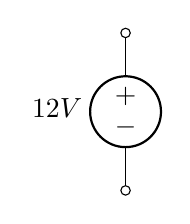
\begin{tikzpicture}[scale=1.00, transform shape, /tikz/circuitikz/bipoles/length=1.50cm, american currents, american voltages, voltage dir=RP]
  \coordinate (1) at (0,2);
  \coordinate (0) at (0,0);
  \draw (0) to [V, l^=${12V}$, n=VIN] (1);
  \draw (1) node[ocirc] {};
  \draw (0) node[ocirc] {};
\end{tikzpicture}
\end{document}